% Figure: the three-job example of Section 1, drawn as two timelines.
% Every number in it is the arithmetic stated in the text of Section~\ref{sec:intro}:
% A = 60 s (stopped at the limit L = 60 s), B = C = 0.2 s, one server, all three
% present at t = 0.  FCFS waits 0 / 60.0 / 60.2 (mean 40.1 s); shortest-first waits
% 0.4 / 0 / 0.2 (mean 0.2 s).  No new computation: this is the paragraph above it.
\begin{figure}[htbp]
\centering
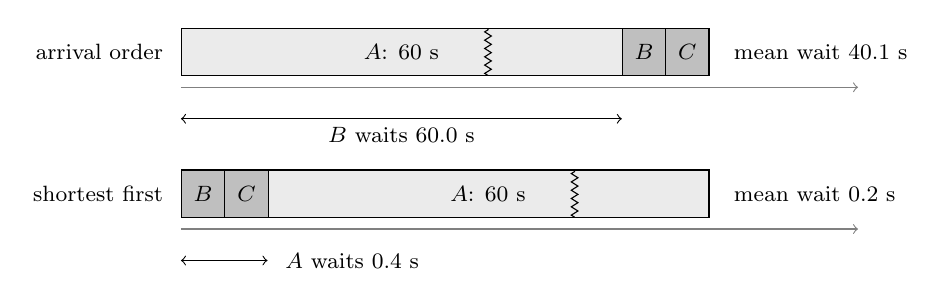
\begin{tikzpicture}[x=1cm,y=1cm,font=\footnotesize]
  % ---- style
  \tikzset{
    jobbox/.style={draw,minimum height=6mm,inner sep=2pt},
    lbl/.style={anchor=east,inner sep=2pt},
  }
  % ---- row 1: arrival order
  \node[lbl] at (-0.15,0.3) {arrival order};
  \draw[->,gray] (0,-0.15) -- (8.6,-0.15);
  \node[jobbox,fill=black!8,minimum width=5.6cm,anchor=west] (a1) at (0,0.3) {};
  \node at (2.8,0.3) {$A$: 60 s};
  % break marks inside A
  \draw[decorate,decoration={zigzag,segment length=3pt,amplitude=1.2pt}] (3.9,0.0) -- (3.9,0.6);
  \node[jobbox,fill=black!25,minimum width=0.55cm,anchor=west] (b1) at (5.6,0.3) {$B$};
  \node[jobbox,fill=black!25,minimum width=0.55cm,anchor=west] (c1) at (6.15,0.3) {$C$};
  \node[anchor=west] at (6.9,0.3) {mean wait 40.1 s};

  % ---- row 2: shortest first
  \node[lbl] at (-0.15,-1.5) {shortest first};
  \draw[->,gray] (0,-1.95) -- (8.6,-1.95);
  \node[jobbox,fill=black!25,minimum width=0.55cm,anchor=west] (b2) at (0,-1.5) {$B$};
  \node[jobbox,fill=black!25,minimum width=0.55cm,anchor=west] (c2) at (0.55,-1.5) {$C$};
  \node[jobbox,fill=black!8,minimum width=5.6cm,anchor=west] (a2) at (1.1,-1.5) {};
  \node at (3.9,-1.5) {$A$: 60 s};
  \draw[decorate,decoration={zigzag,segment length=3pt,amplitude=1.2pt}] (5.0,-1.8) -- (5.0,-1.2);
  \node[anchor=west] at (6.9,-1.5) {mean wait 0.2 s};

  % ---- waits
  \draw[<->] (0,-0.55) -- node[below,inner sep=3pt] {$B$ waits 60.0 s} (5.6,-0.55);
  \draw[<->] (0,-2.35) -- (1.1,-2.35);
  \node[anchor=west,inner sep=2pt] at (1.25,-2.35) {$A$ waits 0.4 s};
\end{tikzpicture}
\caption{The three-job example of Section~\ref{sec:intro} on one server: $A$ is
stopped at the per-job limit $L = \devnum{60}$ s, $B$ and $C$ take
\devnum{0.2} s each, and all three are present at $t = 0$. The boxes are
schematic, not to scale, and the zigzag marks the elided part of $A$. The two
orders execute the same total work; reordering moves \devnum{60} seconds of
waiting off $B$ and $C$ and puts \devnum{0.4} seconds onto $A$. Source: the
arithmetic stated in the text, not a measurement.}
\label{fig:threejob}
\end{figure}
